%% Exemplo de utilizacao do estilo de formatacao normas-utf-tex (http://normas-utf-tex.sourceforge.net)
%% dúvidas acessar o site acima
%%
%%
%% Autores: (200?-2011) Hugo Vieira Neto (hvieir@utfpr.edu.br)
%%          (200?-2011) Diogo Rosa Kuiaski (diogo.kuiaski@gmail.com)
%%          (2011-2017) Marcos Talau <talau@users.sourceforge.net>
%% Colaborador:
%%          (2011) César M. Vargas Benitez <cesarvargasb@gmail.com>

%%
%% IMPORTANTE: O texto está escrito com acentuação antiga, atualmente você
%%             pode escrever acentos sem precisar de códigos para tal.
%%

\documentclass[openright]{normas-utf-tex} %openright = o capitulo comeca sempre em paginas impares
%\documentclass[oneside]{normas-utf-tex} %oneside = para dissertacoes com numero de paginas menor que 100 (apenas frente da folha) 

% force A4 paper format
\special{papersize=210mm,297mm}

\usepackage[alf,abnt-emphasize=bf,bibjustif,recuo=0cm, abnt-etal-cite=2, abnt-etal-list=99]{abntcite} %configuracao correta das referencias bibliograficas.

\usepackage[brazil]{babel} % pacote portugues brasileiro
\usepackage[utf8]{inputenc} % pacote para acentuacao direta
\usepackage{amsmath,amsfonts,amssymb} % pacote matematico
\usepackage{graphicx} % pacote grafico
\usepackage{times} % fonte times
\usepackage[final]{pdfpages} % adicao da ata

%Podem utilizar GEOMETRY{...} para realizar pequenos ajustes das margens. Onde, left=esquerda, right=direita, top=superior, bottom=inferior. P.ex.:
%\geometry{left=3.0cm,right=1.5cm,top=4cm,bottom=1cm} 

% ---------- Preambulo ----------
\instituicao{Universidade Tecnológica Federal do Paraná} % nome da instituicao
\programa{Departamento Acadêmico de Eletrônica} % nome do programa
\area{Informática Industrial} % [Engenharia Biomedica] ou [Informatica Industrial] ou [Telematica]

\documento{Trabalho de Conclusão de Curso}
\nivel{Bacharelado} % [Mestrado] ou [Doutorado]
\titulacao{Bacharel} % [Mestre] ou [Doutor]

\titulo{{zCart: Carrinho de Supermercado Inteligente}} % titulo do trabalho em portugues
\title{\MakeUppercase{zCart: Smart Supermarket Cart}} % titulo do trabalho em ingles

\autor{Flávio Shigueo Miamoto} % autor do trabalho
\autordois{João Pedro Zanlorensi Cardoso} % autor do trabalho
\cita{SOBRENOME, Nome} % sobrenome (maiusculas), nome do autor do trabalho

\palavraschave{Inteligência Artificial, Supermercado, Deep Learning} 
\keywords{Keyword 1, Keyword 2, ...} % palavras-chave do trabalho em ingles

\comentario{\UTFPRdocumentodata\ apresentado ao \UTFPRprogramadata\ da \ABNTinstituicaodata\ como requisito parcial para obtenção do grau de \UTFPRtitulacaodata\ em Engenharia Eletrônica}

\orientador{Prof. Dr. André Eugênio Lazaretti}

\local{Curitiba} % cidade
\data{\the\year} % ano automatico

% desativa hifenizacao mantendo o texto justificado.
% thanks to Emilio C. G. Wille
\tolerance=1
\emergencystretch=\maxdimen
\hyphenpenalty=10000
\hbadness=10000
\sloppy

%---------- Inicio do Documento ----------
\begin{document}

\capa % geracao automatica da capa
\folhaderosto % geracao automatica da folha de rosto

% dedicatoria
\begin{dedicatoria}
Texto da dedicatoria.
\end{dedicatoria}

% agradecimentos (opcional)
\begin{agradecimentos}
Texto dos agradecimentos.
\end{agradecimentos}

% epigrafe (opcional)
\begin{epigrafe}
Texto da epigrafe.
\end{epigrafe}

%resumo
\begin{resumo}
Texto do resumo (maximo de 500 palavras).
\end{resumo}

%abstract
\begin{abstract}
Abstract text (maximum of 500 words).
\end{abstract}

% listas (opcionais, mas recomenda-se a partir de 5 elementos)
\listadefiguras % geracao automatica da lista de figuras
\listadetabelas % geracao automatica da lista de tabelas
\listadequadros % adivinhe :)
\listadesiglas % geracao automatica da lista de siglas
\listadesimbolos % geracao automatica da lista de simbolos

% sumario
\sumario % geracao automatica do sumario


%---------- Inicio do Texto ----------
% recomenda-se a escrita de cada capitulo em um arquivo texto separado (exemplo: intro.tex, fund.tex, exper.tex, concl.tex, etc.) e a posterior inclusao dos mesmos no mestre do documento utilizando o comando \input{}, da seguinte forma:
%\input{intro.tex}
%\input{fund.tex}
%\input{exper.tex}
%\input{concl.tex}

\setcounter{page}{12}

%---------- Primeiro Capitulo ----------
\chapter{Introdução}

O presente documento e um exemplo de uso do estilo de formatacao \LaTeX\ elaborado para atender as Normas para Elaboracao de Trabalhos Academicos da UTFPR. O estilo de formatacao {\ttfamily normas-utf-tex.cls} tem por base o pacote \textsc{abn}\TeX~-- cuja leitura da documentacao \cite{abnTeX2009} e fortemente sugerida~-- e o estilo de formatacao \LaTeX\ da UFPR.

Para melhor entendimento do uso do estilo de formatacao {\ttfamily normas-utf-tex.cls}, aconselha-se que o potencial usuario analise os comandos existentes no arquivo \TeX\ ({\ttfamily modelo\_*.tex}) e os resultados obtidos no arquivo PDF ({\ttfamily modelo\_*.pdf}) depois do processamento pelo software \LaTeX\ + \textsc{Bib}\TeX~\cite{LaTeX2009,BibTeX2009}. Recomenda-se a consulta ao material de referencia do software para a sua correta utilizacao~\cite{Lamport1986,Buerger1989,Kopka2003,Mittelbach2004}.

\begin{quadro}[!htb]
	\centering
	\caption[Exemplo de um quadro]{Exemplo de um quadro mostrando a correlacao entre x e y.}
	\label{tab:correlacao}
	\begin{tabular}{cc}
		\hline 
		x & y \\
		\hline
		1 & 2 \\
		3 & 4 \\
		5 & 6 \\
		7 & 8 \\
		\hline 
	\end{tabular}
	\fonte{Autoria propria.}
\end{quadro}

\section{Motivação}

Uma das principais vantagens do uso do estilo de formatacao {\ttfamily normas-utf-tex.cls} para \LaTeX\ e a formatacao \textit{automatica} dos elementos que comp\~oem um documento academico, tais como capa, folha de rosto, dedicatoria, agradecimentos, epigrafe, resumo, abstract, listas de figuras, tabelas, siglas e simbolos, sumario, capitulos, referencias, etc. Outras grandes vantagens do uso do \LaTeX\ para formatacao de documentos academicos dizem respeito a facilidade de gerenciamento de referencias cruzadas e bibliograficas, alem da formatacao~-- inclusive de equac\~oes  matematicas~-- correta e esteticamente perfeita.

\section{Objetivos}

\subsection{Objetivo Geral}

Prover um modelo de formatacao \LaTeX\ que atenda as Normas para Elaboracao de Trabalhos Academicos da UTFPR~\cite{UTFPR2008} e as Normas de Apresentacao de Trabalhos Academicos do DAELN~\cite{DAELN2006}.

\subsection{Objetivos Específicos}

\begin{itemize}
	\item Obter documentos academicos automaticamente formatados com correcao e perfeicao estetica.
	\item Desonerar autores da tediosa tarefa de formatar documentos academicos, permitindo sua concentracao no conteudo do mesmo.
	\item Desonerar orientadores e examinadores da tediosa tarefa de conferir a formatacao de documentos academicos, permitindo sua concentracao no conteudo do mesmo.
\end{itemize}


%---------- Segundo Capitulo ----------
\chapter{Desenvolvimento}
\label{chap:desenv}

A seguir ilustra-se a forma de incluir figuras, tabelas, equac\~oes, siglas e simbolos no documento, obtendo indexacao automatica em suas respectivas listas. A numeracao sequencial de figuras, tabelas e equac\~oes ocorre de modo automatico. Referencias cruzadas sao obtidas atraves dos comandos {\ttfamily \textbackslash label\{\}} e {\ttfamily \textbackslash ref\{\}}. Por exemplo, nao e necessario saber que o numero deste capitulo e~\ref{chap:desenv} para colocar o seu numero no texto. Isto facilita muito a insercao, remocao ou relocacao de elementos numerados no texto (fato corriqueiro na escrita e correcao de um documento academico) sem a necessidade de renumera-los todos.

\section{Figuras}

Na figura~\ref{fig:dummy} e apresentado um exemplo de grafico flutuante. Esta figura aparece automaticamente na lista de figuras. Para uso avancado de graficos no \LaTeX, recomenda-se a consulta de literatura especializada~\cite{Goossens2007}.


\begin{figure}[!htb]
	\centering
	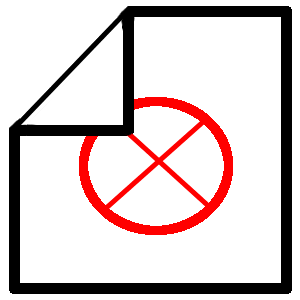
\includegraphics[width=0.2\textwidth]{./dummy.png} % <- formatos PNG, JPG e PDF
	\caption[Exemplo de uma figura]{Exemplo de uma figura onde aparece uma imagem sem nenhum significado especial.}
	\fonte{\cite{abnTeX2009}}
	\label{fig:dummy}
\end{figure}


\section{Tabelas}

Tambem e apresentado o exemplo da tabela~\ref{tab:correlacao}, que aparece automaticamente na lista de tabelas. Informac\~oes sobre a construcao de tabelas no \LaTeX\ podem ser encontradas na literatura especializada~\cite{Lamport1986,Buerger1989,Kopka2003,Mittelbach2004}.

\begin{table}[!htb]
	\centering
	\caption[Exemplo de uma tabela]{Exemplo de uma tabela mostrando a correlacao entre x e y.}
	\label{tab:correlacao}
	\begin{tabular}{cc}
		\hline 
		x & y \\
		\hline
		1 & 2 \\
		3 & 4 \\
		5 & 6 \\
		7 & 8 \\
		\hline 
	\end{tabular}
	\fonte{Autoria propria.}
\end{table}

\section{Equações}

A transformada de Laplace e dada na equacao~(\ref{eq:laplace}), enquanto a equacao~(\ref{eq:dft}) apresenta a formulacao da transformada discreta de Fourier bidimensional\footnote{Deve-se reparar na formatacao esteticamente perfeita destas equac\~oes!}.

\begin{equation}
X(s) = \int\limits_{t = -\infty}^{\infty} x(t) \, \text{e}^{-st} \, dt
\label{eq:laplace}
\end{equation}

\begin{equation}
F(u, v) = \sum_{m = 0}^{M - 1} \sum_{n = 0}^{N - 1} f(m, n) \exp \left[ -j 2 \pi \left( \frac{u m}{M} + \frac{v n}{N} \right) \right]
\label{eq:dft}
\end{equation}

\section{Siglas e símbolos}

O pacote \textsc{abn}\TeX\ permite ainda a definicao de siglas e simbolos com indexacao automatica atraves dos comandos {\ttfamily \textbackslash sigla\{\}\{\}} e {\ttfamily \textbackslash simbolo\{\}\{\}}. Por exemplo, o significado das siglas\sigla{CPGEI}{Programa de Pos-graduacao em Engenharia Eletrica e Informatica Industrial},\sigla{DAELN}{Departamento Academico de Eletronica} e\sigla{UTFPR}{Universidade Tecnologica Federal do Parana} aparecem automaticamente na lista de siglas, bem como o significado dos simbolos\simbolo{$\lambda$}{comprimento de onda},\simbolo{$v$}{velocidade} e\simbolo{$f$}{frequencia} aparecem automaticamente na lista de simbolos. Mais detalhes sobre o uso destes e outros comandos do \textsc{abn}\TeX\ sao encontrados na sua documentacao especifica~\cite{abnTeX2009}.


%---------- Terceiro Capitulo ----------
\chapter{Conclusão}

Espera-se que o uso do estilo de formatacao \LaTeX\ adequado as Normas para Elaboracao de Trabalhos Academicos da UTFPR ({\ttfamily normas-utf-tex.cls}) facilite a escrita de documentos no ambito desta instituicao e aumente a produtividade de seus autores. Para usuarios iniciantes em \LaTeX, alem da bibliografia especializada ja citada, existe ainda uma serie de recursos~\cite{CTAN2009} e fontes de informacao~\cite{TeX-Br2009,Wikibooks2009} disponiveis na Internet.

Recomenda-se o editor de textos Kile como ferramenta de composicao de documentos em \LaTeX\ para usuarios Linux. Para usuarios Windows recomenda-se o editor \TeX nicCenter~\cite{TeXnicCenter2009}. O \LaTeX\ normalmente ja faz parte da maioria das distribuic\~oes Linux, mas no sistema operacional Windows e necessario instalar o software \textsc{MiK}\TeX~\cite{MiKTeX2009}.

Alem disso, recomenda-se o uso de um gerenciador de referencias como o JabRef~\cite{JabRef2009} ou Mendeley~\cite{Mendeley2009} para a catalogacao bibliografica em um arquivo \textsc{Bib}\TeX, de forma a facilitar citac\~oes atraves do comando {\ttfamily \textbackslash cite\{\}} e outros comandos correlatos do pacote \textsc{abn}\TeX. A lista de referencias deste documento foi gerada automaticamente pelo software \LaTeX\ + \textsc{Bib}\TeX\ a partir do arquivo {\ttfamily reflatex.bib}, que por sua vez foi composto com o gerenciador de referencias JabRef.

O estilo de formatacao \LaTeX\ da UTFPR e este exemplo de utilizacao foram elaborados por Diogo Rosa Kuiaski (diogo.kuiaski@gmail.com) e Hugo Vieira Neto (hvieir@utfpr.edu.br), com contribuic\~oes de Cesar Vargas Benitez. Sugest\~oes de melhorias sao bem-vindas.


%---------- Referencias ----------
\clearpage % this is need for add +1 to pageref of bibstart used in 'ficha catalografica'.
\label{bibstart}
\bibliography{reflatex} % geracao automatica das referencias a partir do arquivo reflatex.bib
\label{bibend}

%---------- Apendices (opcionais) ----------
\apendice
\chapter{Nome do Apendice}

Use o comando {\ttfamily \textbackslash apendice} e depois comandos {\ttfamily \textbackslash chapter\{\}}
para gerar titulos de apendices.


% ---------- Anexos (opcionais) ----------
\anexo
\chapter{Nome do Anexo}

Use o comando {\ttfamily \textbackslash anexo} e depois comandos {\ttfamily \textbackslash chapter\{\}}
para gerar titulos de anexos.


% --------- Ordenacao Afabetica da Lista de siglas --------
%\textbf{* Observac\~oes:} a ordenacao alfabetica da lista de siglas ainda nao eh realizada de forma automatica, porem
% eh possivel se de realizar isto manualmente. Duas formas:
%
% ** Primeira forma)
%    A ordenacao eh feita com o auxilio do comando 'sort', disponivel em qualquer
% sistema Linux e UNIX, e tambem em sistemas Windows se instalado o coreutils (http://gnuwin32.sourceforge.net/packages/coreutils.htm)
% comandos para compilar e ordenar, supondo que seu arquivo se chame 'dissertacao.tex':
%
%      $ latex dissertacao
%      $ bibtex dissertacao && latex dissertacao
%      $ latex dissertacao
%      $ sort dissertacao.lsg > dissertacao.lsg.tmp
%      $ mv dissertacao.lsg.tmp dissertacao.lsg
%      $ latex dissertacao
%      $ dvipdf dissertacao.dvi
%
%
% ** Segunda forma)
%\textbf{Sugestao:} crie outro arquivo .tex para siglas e utilize o comando \sigla{sigla}{descricao}.
%Para incluir este arquivo no final do arquivo, utilize o comando \input{arquivo.tex}.
%Assim, Todas as siglas serao geradas na ultima pagina. Entao, devera excluir a ultima pagina da versao final do arquivo
% PDF do seu documento.


%-------- Citacoes ---------
% - Utilize o comando \citeonline{...} para citacoes com o seguinte formato: Autor et al. (2011).
% Este tipo de formato eh utilizado no comeco do paragrafo. P.ex.: \citeonline{autor2011}

% - Utilize o comando \cite{...} para citacoeses no meio ou final do paragrafo. P.ex.: \cite{autor2011}



%-------- Titulos com nomes cientificos (titulo, capitulos e secoes) ----------
% Regra para escrita de nomes cientificos:
% Os nomes devem ser escritos em italico, 
%a primeira letra do primeiro nome deve ser em maiusculo e o restante em minusculo (inclusive a primeira letra do segundo nome).
% VEJA os exemplos abaixo.
% 
% 1) voce nao quer que a secao fique com uppercase (caixa alta) automaticamente:
%\section[nouppercase]{\MakeUppercase{Estudo dos efeitos da radiacao ultravioleta C e TFD em celulas de} {\textit{Saccharomyces boulardii}}
%
% 2) por padrao os cases (maiusculas/minuscula) sao ajustados automaticamente, voce nao precisa usar makeuppercase e afins.
% \section{Introducao} % a introducao sera posta no texto como INTRODUCAO, automaticamente, como a norma indica.


\end{document}

